%%%%%%%%%%%%%%%%%%%%%%%%%%%%%%%
%   Figures for chapter 1
%%%%%%%%%%%%%%%%%%%%%%%%%%%%%%%

\newcommand{\figDrlLocomotionMotivation}{
    \begin{figure}[!ht]
        \centering
        \begin{subfigure}[b]{0.45\textwidth}
            \centering
            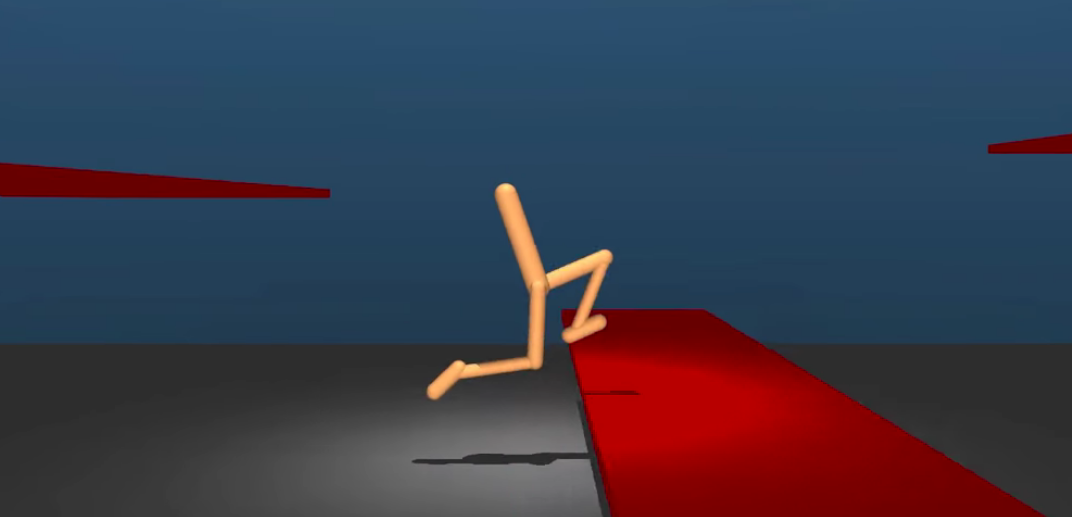
\includegraphics[width=0.9\textwidth]{./chapters/chapter_1/imgs/img_ch1_emergence_of_locomotion.png}
            \caption{}
            \label{fig:ch1_emergence_locomotion}
        \end{subfigure}
        \begin{subfigure}[b]{0.45\textwidth}
            \centering
            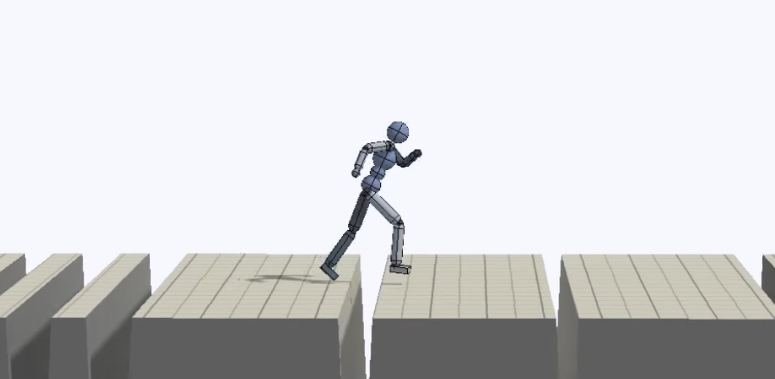
\includegraphics[width=0.9\textwidth]{./chapters/chapter_1/imgs/img_ch1_deepmimic.png}
            \caption{}
            \label{fig:ch1_deepmimic}
        \end{subfigure}
        \caption{Some results from applying Deep Reinforcement Learning to locomotion. 
                    a) Biped traversing simulated environment \citep{DeepmindEmergenceLocomotion}.
                    b) Humanoid traversing simulated environment \citep{DeepMimic} }
        \label{fig:ch1_motivation_drl_locomotion}
    \end{figure}
}